\documentclass{homework}
\usepackage[margin=0.25in]{geometry}
\usepackage{amsmath}
\usepackage{algorithm}
\usepackage{tabularx}
\usepackage{algpseudocode}
\usepackage{graphicx}
\usepackage{svg}
\usepackage{hyperref}
\usepackage[newfloat]{minted}
\usepackage{caption}
\usepackage{etoolbox} % for \ifnumcomp
\usepackage{listofitems} % for \readlist to create arrays
\usepackage{neuralnetwork}
\usepackage{tikz}
\usetikzlibrary{matrix,chains,positioning,decorations.pathreplacing,arrows}
\usepackage{pgf-umlcd}
\usepackage[textwidth=6in]{geometry}
\usepackage[demo]{graphicx}

\newminted{python}{frame=lines,framerule=2pt}
\newenvironment{code}{\captionsetup{type=listing}}{}
\SetupFloatingEnvironment{listing}{name=Output}

\begin{document}

\title{Homework 3 - Multi Layer Perceptron}
\author{Isu Kim 32190984}


\maketitle

\setcounter{section}{-1}
\section{Index}
\label{sec:index}
\begin{enumerate}
    \item Background
    \item Notations and Rules
    \item 1 Hidden Layer with 1 Perceptron
    \item $N$ Hidden Layers with $M$ Perceptrons
    \item $N$ Hidden Layers with $M$ Perceptrons with \textit{ADAM} 
    \item Conclusion
\end{enumerate}

\section{Background}
All the code were verified running in my own private server with following specifications:

\begin{itemize}
  \item \texttt{Python 3.9}
  \item \texttt{Numpy 1.12.5}: For processing math operations.
  \item \texttt{Pandas 1.4.2}: For loading \texttt{.csv} file.
  \item \texttt{Matplotlib 3.5.1}: For visualization.
  \item \texttt{Jupyter Notebook 6.4.8}: For general execution as well as \texttt{.ipynb} file.
\end{itemize}

Honestly speaking, I feel no need for addressing some background knowledge about MLP. For example, what a perceptron is, the XOR problem, why we need MLP instead of single layer and etc. Since I am going to implement MLP from scratch without any help of the internet, we will be dealing with all those math equations in later sections. Therefore, I will keep this background as short as possible. I have provided as much detailed equations and pseudo codes as much as possible and tried to include background knowledge about MLP in the later sections. Therefore, I will close background section here.

\pagebreak

\section{Notations and Rules}
Before we start diving deeper into mathematics, let's make our own notations and our own rules. This is for helping us not lose track of how things work when it gets super complicated.

\subsection{Perceptron}
From now on, I am going to be using following image to denote a perceptron graphically.

\begin{figure}[h]
    \centering
    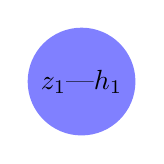
\begin{tikzpicture}[>=latex]
        \path
        % 1st layer
        +(-9.0, 2.0)  node[circle,fill=blue!50,scale=1]  (b1) {$z_{1}$|$h_1$};
    \end{tikzpicture}
    \caption{A Perceptron}
    \label{fig:my_label}
\end{figure}
\\
All the inputs into this perceptron will be summed up as $z_1$. Then with some activation function, this perceptron will have a value of $h_1$. Therefore, this perceptron will also have following equation:

\[
    h_1 = \sigma(z_1)
\]

So, if you see this picture next time in this report, please think it as a perceptron.

\subsection{Weights}
Weights will be noted as $w$. Since we are going to stack layers, an example would be like $w_{12}$. $w_{12}$ will mean that this is the second weight in layer 1.

\subsection{Prediction}
We are going to denote $\hat{y}$ as prediction from our model.

\subsection{Loss Function}
Since this is a regression task, we are going to use \textit{mean squared error} as our loss function for evaluating our model. Therefore the lost function will be defined as following way:

\[
    L = \frac{1}{2}\sum_{i=1}^{m}\{\hat{y} - y^i\}^2
\]
Personally, I find it a lot confusing when using $\delta$ notation. Therefore, I am not going to use $\delta$ notation. Instead, I will be deriving full chain rules. Of course, this will make my equation a lot longer, however at least it does not confuse me. Also, I find it easy to derive chain rules with full notations instead of $\delta$ notation. Furthermore, I am going to mix term "perceptron" and "node". So, when you see "node", please consider it as "perceptron". For validating our model, we are going to use 80\% of the total data as training and the rest of the data as validation data set.

\pagebreak

\section{1 Layer with 1 Perceptron}
\subsection{Model Design}

\begin{figure}[h]
    \centering
    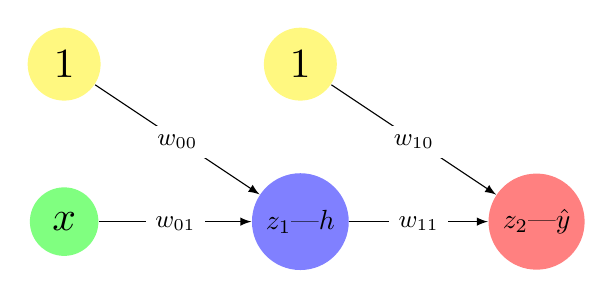
\begin{tikzpicture}[>=latex]
        \path
        % 1st layer
        +(-9.0, 2.0)  node[circle,fill=yellow!50,scale=1.5]  (b1) {$1$}
        +(-9.0, 0)    node[circle,fill=green!50,scale=1.5]  (x) {$x$}
        % 2nd layer
        +(-6.0, 2.0)  node[circle,fill=yellow!50,scale=1.5]  (b2) {$1$}
        +(-6.0, 0)  node[circle,fill=blue!50,scale=1]  (z11) {$z_{1}$|$h$}
        % 3rd layer
        +(-3.0, 0) node[circle,fill=red!50,scale=1]  (y) {$z_2$|$\hat{y}$};

        \draw[->] (b1)--(z11) node[anchor=mid, midway, fill=white]{\small{$w_{00}$}};
        \draw[->] (x)--(z11) node[anchor=mid, midway, fill=white]{\small{$w_{01}$}};

        \draw[->] (b2)--(y) node[anchor=mid, midway, fill=white]{\small{$w_{10}$}};
        \draw[->] (z11)--(y) node[anchor=mid, midway, fill=white]{\small{$w_{11}$}};
    \end{tikzpicture}
    \caption{Model with Single Hidden Layer}
    \label{fig:my_label}
\end{figure}

For extra notations, colors in perceptrons represent the types of each perceptrons. Those are:
\begin{itemize}
    \item \textbf{Yellow}: Bias, this is fixed as 1.
    \item \textbf{Green}: Input, we have $x$.
    \item \textbf{Red}: Output, we have $\hat{y}$.
    \item \textbf{Blue}: Hidden layer.
\end{itemize}

First hidden layer will have single perceptron using \textit{sigmoid} as activation function. Last layer will be a single perceptron using \textit{linear} function as an activation function. As you can see in the picture, the model requires 4 weights to be trained. We are going to use backpropagation with gradient descent in order to fit our model into the data. The code can be found in \texttt{Single_Layer.ipynb}.

\subsection{Math Time}
We love math, right? Since we are going to use gradient descent algorithm in order to train each weights, we need to know following values:
\[
    \frac{\partial L}{\partial w_00}, \quad \frac{\partial L}{\partial w_01}, \quad \frac{\partial L}{\partial w_10}, \quad \frac{\partial L}{\partial w_11}
\]

By using chain rule, we can derive each values easily.

\[
    \begin{aligned}
        \text{a) } &\frac{\partial L}{\partial w_{00}} = \frac{\partial L}{\partial \hat{y}}  \frac{\partial \hat{y}}{\partial z_2}  \frac{\partial z_2}{\partial h}  \frac{\partial h}{\partial z_1}  \frac{\partial z_1}{\partial w_{00}} = (\hat{y} - y) * 1 * w_{11} * \sigma^\prime(z_2) * 1\\
        \text{b) } &\frac{\partial L}{\partial w_{01}} = \frac{\partial L}{\partial \hat{y}} \frac{\partial \hat{y}}{\partial z_2} \frac{\partial z_2}{\partial h} \frac{\partial h}{\partial z_1} \frac{\partial z_1}{\partial w_{01}} = (\hat{y} - y) * 1 * w_{11} * \sigma^\prime(z_2) * x\\
        \text{c) } &\frac{\partial L}{\partial w_{10}} = \frac{\partial L}{\partial \hat{y}} \frac{\partial \hat{y}}{\partial z_2} \frac{\partial z_2}{\partial w_{10}} = (\hat{y} - y) * 1 * 1\\
        \text{d) } &\frac{\partial L}{\partial w_{00}} = \frac{\partial L}{\partial \hat{y}} \frac{\partial \hat{y}}{\partial z_2} \frac{\partial z_2}{\partial w_{11}} = (\hat{y} - y) * 1 * h
    \end{aligned}
\]
\pagebreak
\subsection{Algorithm and Training}
By derived chain rule, we can make following update rules

\[
    \begin{aligned}
    \text{a) } &w_{00} \coloneqq w_{00} - \alpha * (\hat{y} - y) * 1 * w_{11} * \sigma^\prime(z_2) * 1\\
    \text{b) } &w_{01} \coloneqq w_{01} - \alpha * (\hat{y} - y) * 1 * w_{11} * \sigma^\prime(z_2) * x\\
    \text{c) } &w_{10} \coloneqq w_{10} - \alpha * (\hat{y} - y) * 1 * 1\\
    \text{d) } &w_{11} \coloneqq w_{11} - \alpha * (\hat{y} - y) * 1 * h
    \end{aligned}
\]

Since converging all weights will be kind of difficult, I am going to be using number of epochs to determine how long we are going to train the model. Also, let's assume that we have total $n$ data points and we have $m$ epochs to train.

\begin{algorithm}
\caption{Single Hidden Layer}\label{alg:cap}
\begin{algorithmic}
\State $w \gets [1, 1, 1, 1]$ \Comment{Initialize $w$ values}
\For{$j \gets 0$ to $m$}
    \For{$i \gets 0$ to $n$}
        \State Calculate $\hat{y}$ and $h$ \Comment{Forward propagate}
        \State $tmp \gets [0, 0, 0, 0]$
        \State $tmp[0] \gets w[0] - \alpha * (\hat{y} - y) * 1 * w_{11} * \sigma^\prime(z_2) * 1$
        \State $tmp[1] \gets w[1] - \alpha * (\hat{y} - y) * 1 * w_{11} * \sigma^\prime(z_2) * x$
        \State $tmp[2] \gets w[2] - \alpha * (\hat{y} - y) * 1 * 1$
        \State $tmp[3] \gets w[3] - \alpha * (\hat{y} - y) * 1 * h$
        \State $w \gets tmp$ \Comment{Update weights simultaneously}
    \EndFor
\EndFor
\end{algorithmic}
\end{algorithm}

I have implemented this using \texttt{Python} in file \texttt{Single_Layer.ipynb}. Let's fit our model using learning rate as 0.01 and epoch count as 10. Then, we get following output from code:
\\
\begin{center}
\begin{code}
\begin{minted}[frame=single,framesep=10pt]{bash}
====================
Alpha: 0.01
Epoch: 10
====================
Epoch 0 / Validation Loss = 1.075299756237752e+02
Epoch 1 / Validation Loss = 1.0512681424065983e+02
...
Epoch 7 / Validation Loss = 1.0490193633776822e+02
Epoch 8 / Validation Loss = 1.0490264099492357e+02
Epoch 9 / Validation Loss = 1.0490295461857167e+02
\end{minted}
\captionof{listing}{Single Layer Training}
\end{code}
\end{center}
\pagebreak
For each weight values, we can get following values:
\begin{center}
\begin{table}[h]
\begin{tabularx}{1.0\textwidth} { 
  | >{\centering\arraybackslash}X 
  | >{\centering\arraybackslash}X 
  | >{\centering\arraybackslash}X 
  | >{\centering\arraybackslash}X | }
 \hline
 $w_{00}$ & $w_{01}$ & $w_{10}$ & $w_{11}$\\
 \hline
 -1.778770819375 & -0.16241236287347 & -5.654484046435 & -2.4095863653231\\
\hline
\end{tabularx}
\caption{Weights with Single Hidden Layer}
\end{table}
\end{center}
Now, let's check how our trained model is visualized compared to the real data.

\begin{figure}[h]
  \centering
  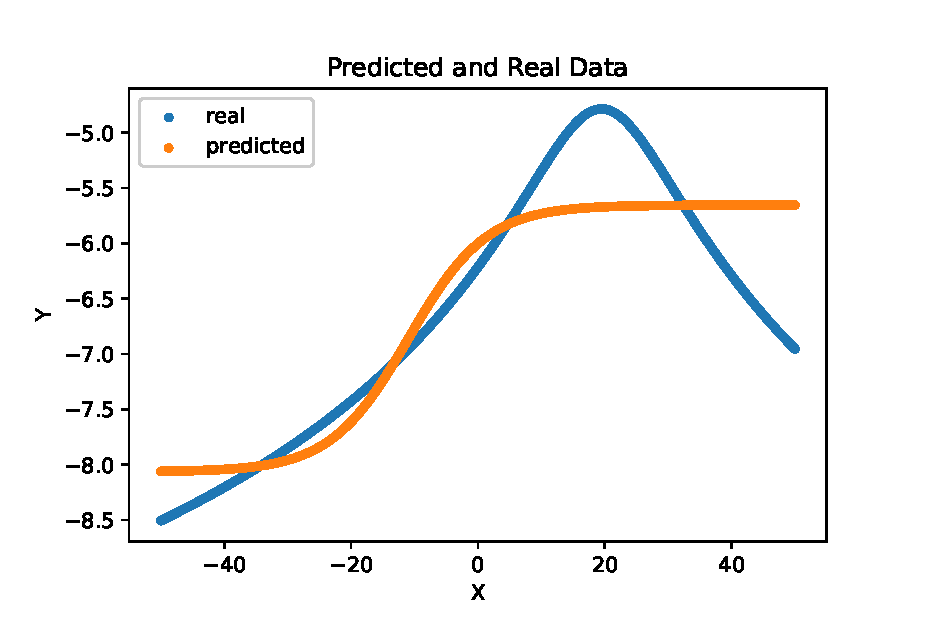
\includegraphics[scale=0.8]{single_layer.eps}
  \caption{Model Representation}
\end{figure}

Since there was only one hidden layer, the graph followed \textit{sigmoid} function. For validation loss, we got value of roughly 104.



\subsection{Comparison with \texttt{TensorFlow}}
For validating our model, let's compare our model with the one generated by professional machine learning library. Among lots of libraries, I have used \texttt{TensorFlow} to check how it performed. With the same conditions, same number of layers and perceptrons, the model was trained by \texttt{TensorFlow}. The code using \texttt{TensorFlow} is not attached to the file that was submitted. With \texttt{TensorFlow}, we could get following weight values:

\begin{center}
\begin{table}[h]
\begin{tabularx}{1.0\textwidth} { 
  | >{\centering\arraybackslash}X 
  | >{\centering\arraybackslash}X 
  | >{\centering\arraybackslash}X 
  | >{\centering\arraybackslash}X | }
 \hline
 $w_{00}$ & $w_{01}$ & $w_{10}$ & $w_{11}$\\
 \hline
 -1.4594318 & -0.12608556 & -2.6065066 & -5.58892\\
\hline
\end{tabularx}
\caption{Weights by \texttt{TensorFlow}}
\end{table}
\end{center}
\pagebreak
For the representation of model's prediction and real data, it was like following graph:
\begin{figure}[h]
  \centering
  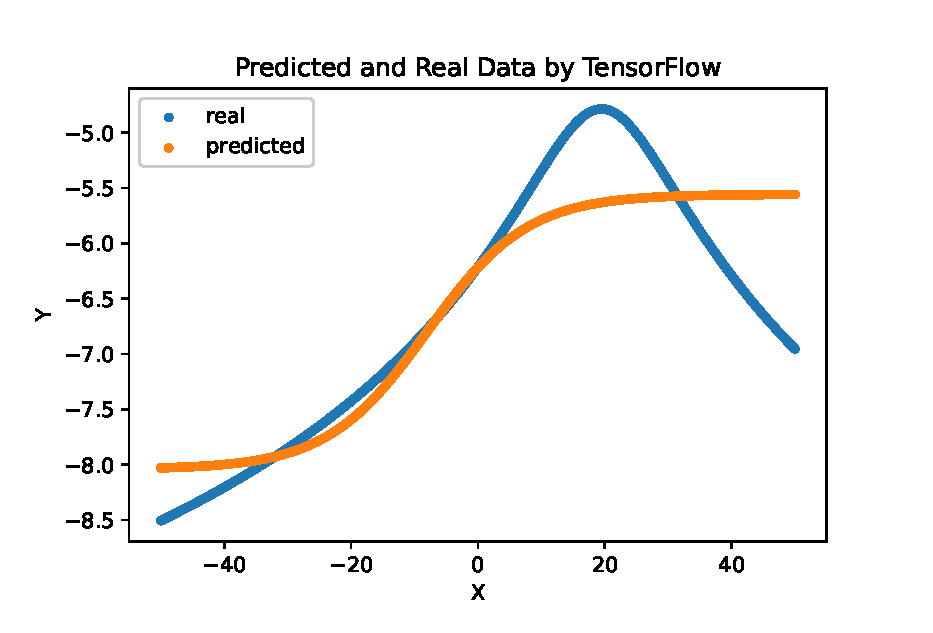
\includegraphics[scale=0.8]{tf_single_layer.eps}
  \caption{Model Representation by \texttt{TensorFlow}}
\end{figure}
\\
\\
The problem with those two models is that they have just one single hidden layer. Since the hidden layer's activation function is sigmoid function and the last activation function is linear function, it is obvious fact that the model will be shaped based upon a sigmoid function. However, as we all know, the data that professor gave us does not fit perfectly into sigmoid function. Therefore, since we have tasted how to implement MLP, let's implement more complex model with more layers. The journey of implementing complex models will be dealt in the next page.
\pagebreak

\section{$N$ Hidden Layers with $M$ Perceptrons}
So with not so deep layers, I actually derived chain rule myself and fed it into my program. However, with some deep layers, we can't. For example, if we had 4 hidden layers with each having 5 perceptrons, each layer would have 20 weights to update. That is impossible for me to calculate and feed it into the program. Also, deriving shallow chain rule was simple. However, with deep chain rules which involves multiple chain rules being added together, it is almost impossible to calculate it by hand. Therefore, we need to make an algorithm that automatically derives chain rule and calculate the value on its on.

\begin{figure}[h]
    \centering
    \begin{tikzpicture}[>=latex]
        \path
        % 1st layer
        +(-9.0, 2.0)  node[circle,fill=yellow!50,scale=1.5]  (b1) {$1$}
        +(-9.0, 0)    node[circle,fill=green!50,scale=1.5]  (x) {$x$}
        % 2nd layer
        +(-6.0, 2.0)  node[circle,fill=yellow!50,scale=1.5]  (b2) {$1$}
        +(-6.0, 0)  node[circle,fill=blue!50,scale=1.5]  (z11) {$z_{11}$}
        +(-6.0, -2.0)  node[circle,fill=blue!50,scale=1.5]  (z12) {$z_{12}$}
        % 3rd layer
        +(-3.0, 2.0)  node[circle,fill=yellow!50,scale=1.5]  (b3) {$1$}
        +(-3.0, 0)  node[circle,fill=blue!50,scale=1.5]  (z21) {$z_{21}$}
        +(-3.0, -2.0)  node[circle,fill=blue!50,scale=1.5]  (z22) {$z_{22}$}
        % 4th layer
        +(+0.0, 2.0)  node[circle,fill=yellow!50,scale=1.5]  (b4) {$1$}
        +(+0.0, 0)  node[circle,fill=blue!50,scale=1.5]  (z31) {$z_{31}$}
        +(+0.0, -2.0)  node[circle,fill=blue!50,scale=1.5]  (z32) {$z_{32}$}

        +(+3.0, 0) node[circle,fill=red!50,scale=1.5]  (y) {$\hat{y}$};

        \draw[->] (b1)--(z11) node[anchor=mid, midway]{\small{$w_{00}$}};
        \draw[->] (b1)--(z12) node[anchor=mid, midway, above left=5mm of z12 and 1mm of z12]{\small{$w_{01}$}};
        \draw[->] (x)--(z11) node[anchor=mid, midway, below right=1.1mm of x and 1mm of x]{\small{$w_{02}$}};
        \draw[->] (x)--(z12) node[anchor=mid, midway]{\small{$w_{03}$}};

        \draw[->] (b2)--(z21) node[anchor=mid, midway]{\small{$w_{10}$}};
        \draw[->] (b2)--(z22) node[anchor=mid, midway, above left=5mm of z22 and 1mm of z22]{\small{$w_{11}$}};
        \draw[->] (z11)--(z21) node[anchor=mid, midway, midway]{\small{$w_{12}$}};
        \draw[->] (z11)--(z22) node[anchor=mid, midway, midway]{\small{$w_{13}$}};
        \draw[->] (z12)--(z21) node[anchor=mid, midway, above right=1.1mm of z12 and 1mm of z12]{\small{$w_{14}$}};
        \draw[->] (z12)--(z22) node[anchor=mid, midway]{\small{$w_{15}$}};

        \draw[->] (b3)--(z31) node[anchor=mid, midway]{\small{$w_{20}$}};
        \draw[->] (b3)--(z32) node[anchor=mid, midway, above left=5mm of z32 and 1mm of z32]{\small{$w_{21}$}};
        \draw[->] (z21)--(z31) node[anchor=mid, midway]{\small{$w_{22}$}};
        \draw[->] (z21)--(z32) node[anchor=mid, midway]{\small{$w_{23}$}};
        \draw[->] (z22)--(z31) node[anchor=mid, midway, above right=1.1mm of z22 and 1mm of z22]{\small{$w_{24}$}};
        \draw[->] (z22)--(z32) node[anchor=mid, midway]{\small{$w_{25}$}};

        \draw[->] (b4)--(y) node[anchor=mid, midway]{\small{$w_{30}$}};
        \draw[->] (z31)--(y) node[anchor=mid, midway]{\small{$w_{31}$}};
        \draw[->] (z32)--(y) node[anchor=mid, midway]{\small{$w_{32}$}};
        
    \end{tikzpicture}
    \caption{Example Network with 3 Hidden Layers}
    \label{fig:my_label}
\end{figure}

This single network image took me 2 hours to draw using \texttt{tikzpicture} in \texttt{LaTeX}, I sincerely regret drawing this. Since I had to express every weights, the graph got a lot messy. Also, please understand that $h_{mn}$ was removed from the picture since there was no enough room for that. Let's take a look at the model and try to actually find patterns on how each chain rules are derived.

To generalize process of deriving chain rules, let's take some example chain rules. From now on, we are going to see a list of chain rules with simple examples from the graph above.
\subsection{Depth 1 Chain Rule}
\begin{figure}[h]
    \centering
    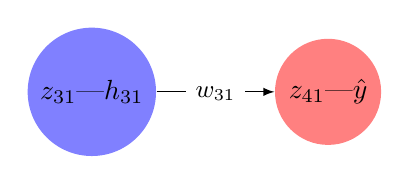
\begin{tikzpicture}[>=latex]
        \path
        % 4th layer
        +(+0.0, 0)  node[circle,fill=blue!50,scale=1]  (z31) {$z_{31}$|$h_{31}$}
        +(+3.0, 0) node[circle,fill=red!50,scale=1]  (y) {$z_{41}$|$\hat{y}$};
        \draw[->] (z31)--(y) node[anchor=mid, midway, fill=white]{\small{$w_{31}$}};
    \end{tikzpicture}
    \caption{Depth 1 Chain Rule}
    \label{fig:my_label}
\end{figure}

For updating $w_{31}$, following chain rule will be used:
\[
    \frac{\partial L}{\partial w_{31}} = \frac{\partial L}{\partial \hat{y}} \frac{\partial \hat{y}}{\partial z_{41}}\frac{\partial z_{41}}{\partial z_{31}} = (\hat{y} - y)*1*h_{31} 
\]
This chain rule can be easily derived since the the weight $w_{31}$ does not affect other weights or other perceptrons. So, let's take a look at some examples that affect other weights and other perceptrons.

\pagebreak
\subsection{Depth 2 Chain Rule}
\begin{figure}[h]
    \centering
    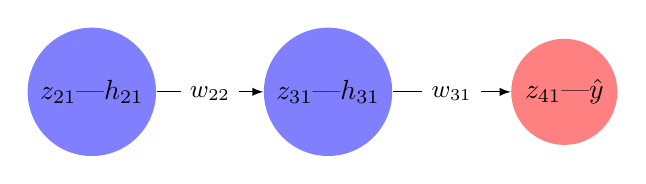
\begin{tikzpicture}[>=latex]
        \path
    
        % 3rd layer
        +(-3.0, 0)  node[circle,fill=blue!50,scale=1]  (z21) {$z_{21}$|$h_{21}$}
        % 4th layer
        +(+0.0, 0)  node[circle,fill=blue!50,scale=1]  (z31) {$z_{31}$|$h_{31}$}
        +(+3.0, 0) node[circle,fill=red!50,scale=1]  (y) {$z_{41}$|$\hat{y}$};

        \draw[->] (z21)--(z31) node[anchor=mid, midway,fill=white]{\small{$w_{22}$}};

        \draw[->] (z31)--(y) node[anchor=mid, midway, fill=white]{\small{$w_{31}$}};
    \end{tikzpicture}
    \caption{Depth 2 Chain Rule}
    \label{fig:my_label}
\end{figure}

For updating $w_{22}$, following chain rule will be used:
\[
    \frac{\partial L}{\partial w_{22}} = \frac{\partial L}{\partial \hat{y}} \frac{\partial \hat{y}}{\partial z_{41}}\frac{\partial z_{41}}{\partial h_{31}}\frac{\partial h_{31}}{\partial z_{31}}\frac{\partial z_{31}}{\partial w_{22}} = (\hat{y} - y)*1*w_{31}*\sigma^\prime(z_{31})*h_{21} 
\]

Since $w_{22}$ affects node $z_{31}$ and weight $w_{31}$, this gets a bit complicated. However, this is a simple form of chain rule since the node $z_{31}$ does not affect any other nodes. So, let's take a look at more complicated ones.

\subsection{Depth 3 Chain Rule}

\begin{figure}[h]
    \centering
    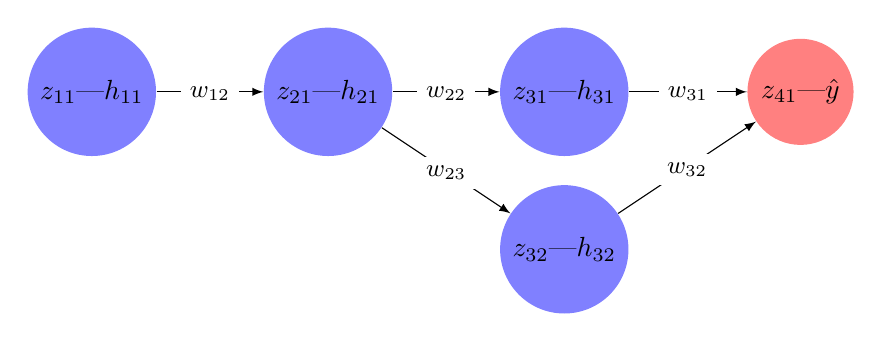
\begin{tikzpicture}[>=latex]
        \path
        % 2nd layer
        +(-6.0, 0)  node[circle,fill=blue!50,scale=1]  (z11) {$z_{11}$|$h_{11}$}
        % 3rd layer
        +(-3.0, 0)  node[circle,fill=blue!50,scale=1]  (z21) {$z_{21}$|$h_{21}$}
        % 4th layer
        +(+0.0, 0)  node[circle,fill=blue!50,scale=1]  (z31) {$z_{31}$|$h_{31}$}
        +(+0.0, -2.0)  node[circle,fill=blue!50,scale=1]  (z32) {$z_{32}$|$h_{32}$}
        +(+3.0, 0) node[circle,fill=red!50,scale=1]  (y) {$z_{41}$|$\hat{y}$};
        \draw[->] (z11)--(z21) node[anchor=mid, midway, fill=white]{\small{$w_{12}$}};
       
        \draw[->] (z21)--(z31) node[anchor=mid, midway, fill=white]{\small{$w_{22}$}};
        \draw[->] (z21)--(z32) node[anchor=mid, midway, fill=white]{\small{$w_{23}$}};

        \draw[->] (z31)--(y) node[anchor=mid, midway, fill=white]{\small{$w_{31}$}};
        \draw[->] (z32)--(y) node[anchor=mid, midway, fill=white]{\small{$w_{32}$}};
        
    \end{tikzpicture}
    \caption{Example Netork with 3 Hidden Layers}
    \label{fig:my_label}
\end{figure}
For updating $w_{12}$, following chain rule will be used:
\begin{multline}
    \frac{\partial L}{\partial w_{12}} = \frac{\partial L}{\partial \hat{y}} \frac{\partial \hat{y}}{\partial z_{41}} \Big\{ \frac{\partial z_{41}}{\partial h_{31}} \frac{\partial h_{31}}{\partial z_{31}} \frac{\partial z_{31}}{\partial h_{21}} + \frac{\partial z_{41}}{\partial h_{32}} \frac{\partial h_{32}}{\partial z_{32}} \frac{z_{32}}{\partial h_{21}} \Big\}\frac{\partial h_{21}}{\partial z_{21}} \frac{\partial z_{21}}{\partial w_{12}} = \\ (\hat{y} - y)*1*\{w_{31}*\sigma^\prime(z_{31})*h_{21} + w_{32}*\sigma^\prime(z_{32})*h_{21}\} * \sigma^\prime(z_{21})*h_{11} \notag
\end{multline}

This is complicated right? There are two routes that $w_{12}$ affects the total loss $L$.
\begin{itemize}
    \item $h_{11} \rightarrow z_{21} \rightarrow z_{31} \rightarrow z_{41} \rightarrow L$
    \item $h_{11} \rightarrow z_{21} \rightarrow z_{32} \rightarrow z_{41} \rightarrow L$
\end{itemize}

Since one weight affects next perceptron and the perceptron after that perceptron, there are lots of elements that are affecting $w_{12}$. Therefore, this gets super complicated. However, if you take a close look at those three examples, there seems to be a pattern.
\pagebreak

\subsection{Rules}\label{rules}
This rule is a rule that I found. Not the one that I looked up Google. Therefore, this rule might be totally wrong. Let's see those chain rules again:

\[
    \begin{aligned}
        \text{a) } &\frac{\partial L}{\partial w_{31}} = (\hat{y} - y)*1*h_{31} \\
        \text{b) } &\frac{\partial L}{\partial w_{22}} = (\hat{y} - y)*1*w_{31}*\sigma^\prime(z_{31})*h_{21} \\
        \text{c) } &\frac{\partial L}{\partial w_{12}} = (\hat{y} - y)*1*\{w_{31}*\sigma^\prime(z_{31})*h_{21} + w_{32}*\sigma^\prime(z_{32})*h_{21}\} * \sigma^\prime(z_{21})*h_{11}
    \end{aligned}
\]

All those three equations all have a common pattern. So, for demonstration let's assume following case:
\begin{figure}[h]
    \centering
    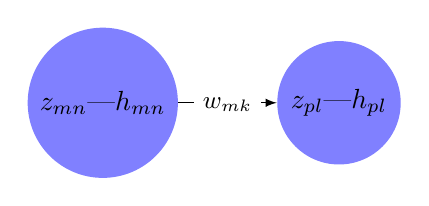
\begin{tikzpicture}[>=latex]
        \path
        % 4th layer
        +(+0.0, 0)  node[circle,fill=blue!50,scale=1]  (z31) {$z_{mn}$|$h_{mn}$}
        +(+3.0, 0) node[circle,fill=blue!50,scale=1]  (y) {$z_{pl}$|$h_{pl}$};
        \draw[->] (z31)--(y) node[anchor=mid, midway, fill=white]{\small{$w_{mk}$}};
    \end{tikzpicture}
    \caption{Example Node}
    \label{fig:my_label}
\end{figure}

When we are going to update weight $w_{mk}$ which is an weight of node with $z_{mn}$, it satisfies following statement:
\[
    \frac{\partial L}{\partial w_{mk}} = (\hat{y} - y) * 1 * V * h_{mn}, \quad V \text{will be dealt later}
\]

Retrieving $V$ is the difficult part. As you can see $V$ is actually the result of chain rule calculation before current perceptron. Meaning that if we need to get $V$, we need to add all backpropagation results from all those perceptrons and weights that current weight $w_{mk}$ is affecting. However, when we think of a chain rule, it is basically a simple recursive function. By deriving a simple recurrence relation, we can derive following recursive function:

\begin{algorithm}
\caption{Recursive Function for Chain Rule}\label{alg:cap}
\begin{algorithmic}
\Procedure{Recursive}{$curNode$}
\If{$curNode$ has no next node}  \Comment{Terminal condition}
    \State return 1
\Else 
    \State $sum \gets 0$
    \State $h \gets curNode$'s $h$ value.
    \State $z \gets curNode$'s $z$ value.
    \State $tmp \gets 0$ 
    \State $weights \gets curNode.weights$
    \For{$i \gets 0$ to $weights$ count} \Comment{Calculate chain rule recursively}
        \State $tmp \gets tmp + Recursive(weights[i].toNode) * weights[i].value$ 
    \EndFor
    \State return $tmp * curNode.activation^\prime(z)$
\EndIf
\end{algorithmic}
\end{algorithm}

\pagebreak
So the algorithms can be found. So let's try to implement this using \texttt{Python}. I personally considered implementing this full feature in \texttt{C++} or \texttt{C} due to the computation speed. Since \texttt{Python} normally performs worse than \texttt{C} or \texttt{C++}, stacking multiple layers will make huge difference. However, due to some powerful libraries of \texttt{Python}, I have decided to implement this using \texttt{Python}. Also, in order for this program to be easily implemented with the algorithm that I have devised, I have chosen OOP style code to implement the whole project. Of course, the overhead of calling functions between different objects might have higher overhead than using just a single matrix, using classes will make the program more intuitive than not using it. In order to make our program, we need following classes.

\begin{itemize}
    \item \texttt{Node}: For storing node (perceptron).
    \item \texttt{Weight}: For storing weight.
    \item \texttt{Layer}: For storing weights and nodes as a layer.
    \item \texttt{Network}: For storing multiple layers and actually performing ML.
\end{itemize}

Let's see how each classes are defined by UML Class Diagram.

\subsection{Design}
All the implementation of this classes can be found under \texttt{MultiLayer.ipynb}. Each classes were designed in a way that can maximize polymorphism and encapsulation as much as possible. Since I would like to mimic functions that are from \texttt{TensorFlow}, I borrowed some function names from \texttt{TensorFlow}. Since each functions are designed in a way that was supposed to work for only this program, the same implementation might not work in some other programs.

\begin{figure}[h]
\centering
    \begin{tikzpicture}
      \begin{class}[text width=16cm]{Network}{0,0}
        \attribute{+ layers: \texttt{List<Layer>}}
        \operation{+ predict(\texttt{Float x})}
        \operation{+ fit(\texttt{List<Float> x_data}, \texttt{List<Float> y_data}), \texttt{Int epoch}, \texttt{Float learning_rate})}
        \operation{+ get_cost(\texttt{List<Float> x_data}, \texttt{List<Float> y_data})}
        \operation{- _forward_propagate(\texttt{Float x})}
        \operation{- _r_get_chain_rules(\texttt{Node cur_node})}
        \operation{- _back_propagate(\texttt{Float x}, \texttt{Float y}, \texttt{Float learning_rate})}
      \end{class}
    \end{tikzpicture}
    \caption{UML Class Diagram for \texttt{Network}}
\end{figure}

This is the most important class. This class will manage the whole MLP and all its necessary information. From initializing all nodes and weights to training weights and predicting values, this class works as a framework for the whole MLP. This class internally has following methods to operate:

\begin{itemize}
    \item \texttt{_forward_propagate}: The methods that forward propagates. This will set all $z$ and $h$ vales to all nodes.
    \item \texttt{_back_propagate}: The methods that backpropagate with the provided $x$ and $y$ pair with learning rate. This methods will internally call \texttt{_forward_propagate} before backpropagating. 
    \item \texttt{_r_get_chain_rules}: The methods that solves chain rules. As mentioned in \hyperref[rules]{section 4.4}, this methods will calculate all chain rule values that is needed when backpropagating. This methods works in a recursive way.
\end{itemize}

Due to \texttt{Python}'s limitations on recursive functions, the maximum depth that \texttt{_r_get_chain_rules} can dive into is limited to 1,000 by default. If you are planning to stack more layers, please set  \texttt{Pyhton}'s maximum recursion depth by using \texttt{sys.setrecursionlimit}. However this is not suggested since deeper layers in this program will usually run very slow. Those three listed methods are internally used methods, meaning that using each methods were not designed to be user-friendly. For user-friendly methods, the list is as it follows:
\begin{itemize}
    \item \texttt{predict}: The method that predicts value with input x. 
    \item \texttt{fit}: The method that fits the model into the provided data. 
    \item \texttt{get_cost}: The method that calculates cost of the model with provided dataset.
\end{itemize}

Also, this class will automatically generate weights connecting each nodes when initializing. Meaning that if you are to use bare \texttt{Layer} class, no weights will be connected to nodes. Therefore, if you wish to see each layers and its weight values, please make a new \texttt{Network} class and take a look inside the network.

\begin{figure}[h]
\centering
    \begin{tikzpicture}
      \begin{class}[text width=16cm]{Layer}{0,0}
        \attribute{- activation: \texttt{String}}
        \attribute{+ nodes: \texttt{List<Node>}}
        \attribute{+ weights: \texttt{List<Weight>}}
        \attribute{+ layer_index: \texttt{Int}}
        \attribute{+ is_output_layer: \texttt{Bool}}
        \operation{+ set_weights(\texttt{List<Weight weights>})}
      \end{class}
    \end{tikzpicture}
    \caption{UML Class Diagram for \texttt{Layer}}
\end{figure}

This class is for generating each layers. However since this is an internal class that is required for the class \texttt{Network} to operate properly, this is not so user-friendly class. As mentioned above, please use \texttt{Network} class for user purpose. When the class's \texttt{__repr__} method was called, this will return an example like below showing the status of current layer.
\\
\begin{center}
\begin{code}
\begin{minted}[frame=single,framesep=10pt]{python}
===== Layer 1 =====
Activiation: linear
Node Count (Including Bias): 6
Weight Count: 30
\end{minted}
\captionof{listing}{Example Output for \texttt{Layer}}
\end{code}
\end{center}
This will tell you a brief information on the layer's status. If you need to see detailed information on its weights and nodes, please check \texttt{Layer.nodes} and \texttt{Layer.weights} for specific values.

\pagebreak

\begin{figure}[h]
\centering
    \begin{tikzpicture}
      \begin{class}[text width=16cm]{Node}{0,0}
        \attribute{+ h: \texttt{Float}}
        \attribute{+ z: \texttt{Float}}
        \attribute{+ layer_count: \texttt{Int}}
        \attribute{+ node_count: \texttt{String}}
        \attribute{+ weights: \texttt{List<Weight>}}
        \attribute{+ neighbors: \texttt{List<Node>}}
        \attribute{- activation: \texttt{String}}
        \operation{+ refresh_weights()}
        \operation{+ get_derivative_z()}
        \operation{+ get_neighbors()}
        \operation{+ calc_h()}
      \end{class}
    \end{tikzpicture}
    \caption{UML Class Diagram for \texttt{Node}}
\end{figure}

This class is for representing a single perceptron. This class has following methods:
\begin{itemize}
    \item \texttt{refresh_weights}: When the \texttt{Node} is initialized, it does not store any weights at all. When \texttt{Network} finishes generating all nodes, it will connect all nodes one by one sequentially. After \texttt{Network} has set weights to all nodes, this method will automatically set the \texttt{Node}'s weight value accordingly.
    \item \texttt{get_derivative_z}: This method returns the value of $\sigma^\prime(z)$. This method is used when deriving chain rules.
    \item \texttt{get_neighbors}: This method returns the connected nodes of current node. This was supposed to be used, however is not used at all.
    \item \texttt{calc_h}: This method calculates $h$ value from $z$ by calculating $h = \sigma(z)$. This function will store $h$ value internally. This method is used for forward propagation.
\end{itemize}

All those methods were not meant to be called individually. Therefore, using those methods alone will not work properly.

\begin{figure}[h]
\centering
    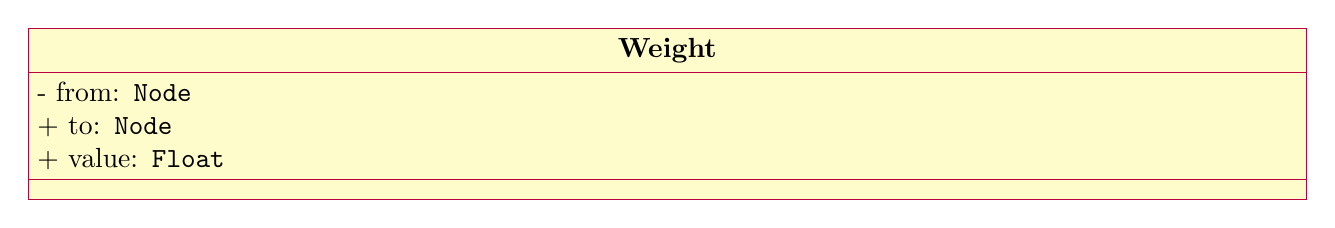
\begin{tikzpicture}
      \begin{class}[text width=16cm]{Weight}{0,0}
        \attribute{- from: \texttt{Node}}
        \attribute{+ to: \texttt{Node}}
        \attribute{+ value: \texttt{Float}}
      \end{class}
    \end{tikzpicture}
    \caption{UML Class Diagram for \texttt{Weight}}
\end{figure}

This class is for representing a weight. \texttt{Weight} does not have any connection when this was first initialized. \texttt{Network} connects all \texttt{Weight}s to \texttt{Node}s. Also, the initial value of weight will be set randomly using \texttt{random.random()}. Therefore, the initial value will be a random \texttt{Float} value from 0 to 1.0. Since this value is initialized randomly, even with the same network setting with the same arguments might have different fitting results for the data. 

\pagebreak

\subsection{Usage}
The program supports a list of activiation functions. Those are the activation functions that are supported:
\begin{itemize}
    \item \texttt{linear}: Identity function
    \item \texttt{sigmoid}: Sigmoid function
    \item \texttt{relu}: ReLU function
    \item \texttt{tanh}: Hyperbolic Tangent
\end{itemize}

In order to generate a new network, you need to use \texttt{Network} class. \texttt{Network} takes two \texttt{tuple} arguments.
\begin{enumerate}
    \item \texttt{layer_node_counts}: Each layer's node counts. If you are going to use 3 layers in 1st hidden layer, 5 nodes in 2nd hidden layer, you should set it as \texttt{(1, 3, 5, 1)}.
    \item \texttt{layer_activation_functions}: Each layer's activation functions. If you are going to use \texttt{sigmoid} and \texttt{relu} as your activation functions in 1st hidden layer and 2nd hidden layer, you should set it as \texttt{('linear', 'sigmoid', 'relu', 'linear')}.
\end{enumerate}
We need to put input layer and output layer by manual. Therefore, we need extra two more layers. Please be aware of this issue. So an example would be :
\\
\begin{center}
    \texttt{Network((1,2,1), ('linear', 'sigmoid', 'linear'))}    
\end{center}
This will generate a network with one hidden layer with its activation function as sigmoid function. Please keep in mind that you need to put input and output layer manually. \texttt{Network} includes \texttt{__repr__} function which describes the whole network. An example output is like below.
\\
\begin{center}
\begin{code}
\begin{minted}[frame=single,framesep=10pt]{python}
>> n1= Network((1,2,1), ('linear', 'sigmoid', 'linear'))
>> print(n1)
===== Layer 1 =====
Activiation: linear
Node Count (Including Bias): 2
Weight Count: 4
===== Layer 2 =====
Activiation: sigmoid
Node Count (Including Bias): 3
Weight Count: 3
===== Layer 3 =====
Activiation: linear
Node Count (Including Bias): 1
Weight Count: 0
===== Output =====
\end{minted}
\captionof{listing}{Representation of \texttt{Network}}
\end{code}
\end{center}
\\
Looks similar to \texttt{TensorFlow} right? Since we include bias term automatically, there will be one more perceptron in each layers. Also, since the program supports no limited combination of each activity functions, you can mix match all activation functions and the layer's perceptron counts as well. 

Let's fit our model into \texttt{hw3_data.csv} using 10 epochs with learning rate of 0.01. We are going to use a single hidden layer with two perceptrons which uses sigmoid function as activiation function.
\\

\begin{center}
\begin{code}
\begin{minted}[frame=single,framesep=10pt]{python}
>> n1.fit(x, y, 10, 0.01)
>> print(n1)
Epoch 0 | 10 / Training Loss : 6.056653080994851e+02
Epoch 1 | 10 / Training Loss : 5.254607179252558e+02
Epoch 2 | 10 / Training Loss : 4.975042169655134e+02
Epoch 3 | 10 / Training Loss : 4.636989838836882e+02
Epoch 4 | 10 / Training Loss : 4.2164048489411016e+02
Epoch 5 | 10 / Training Loss : 3.756166273890967e+02
Epoch 6 | 10 / Training Loss : 3.332303765747995e+02
Epoch 7 | 10 / Training Loss : 3.11146985127094e+02
Epoch 8 | 10 / Training Loss : 3.123465111127894e+02
Epoch 9 | 10 / Training Loss : 3.188713945954729e+02
\end{minted}
\captionof{listing}{Example Code Fitting \texttt{Network}}
\end{code}
\end{center}

The loss is calculated using MSE. As you can see, the training error gets lower after each epochs! You can predict a value by using \texttt{Network.predict()}. For all $x$s in \texttt{hw3_data.csv}, let's compare the prediction of this model and the original data. 

\begin{figure}[h]
  \centering
  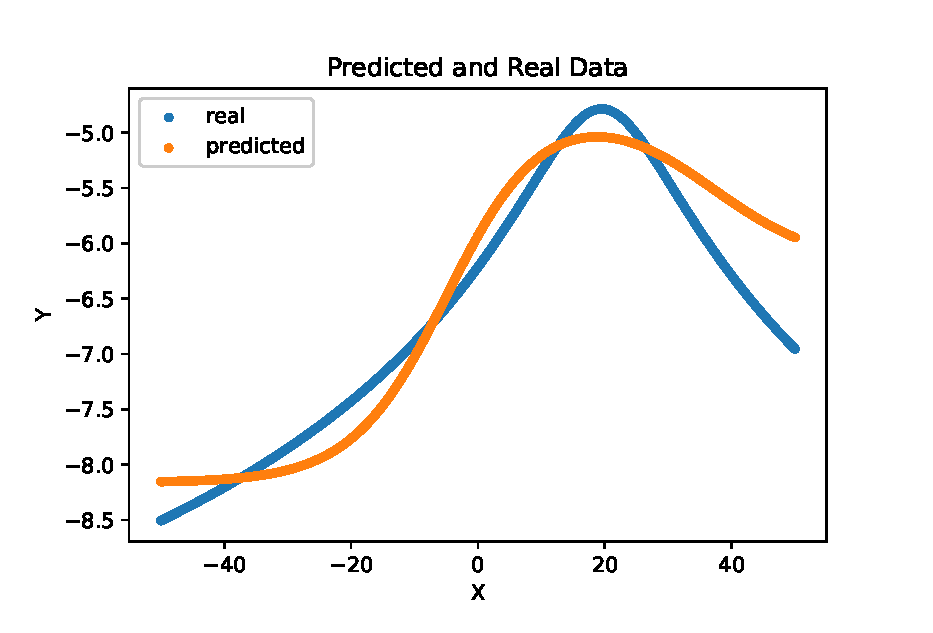
\includegraphics[scale=0.7]{multi_layer_demo_1.eps}
  \caption{MLP Fitting Example}
\end{figure}

This seems okay to me. For validation loss, it had value of roughly 63 which is better than the one that we have used last time with section 3.3 (it had value of 104). Since this is just one hidden layer with two perceptrons, let's try much more complex models and test if our program actually works. 
\pagebreak

\subsection{Overfitting}

Since I have implemented MLP program, let's play with the models by tuning some parameters and arguments. We have a variety of parameters to play with:

\begin{itemize}
    \item Learning rate
    \item Epochs
    \item Activation functions per layer
    \item Node counts per layer
\end{itemize}

Since my program supports customization of all parameters, we can make any combination that we would like to test. From now on, I have decided to make my program generate a model that fits the most out of the real data. Of course, overfitting is not a good thing, however this will actually prove that my program works without any problems. Also, watching my program generate models would be a fun thing to watch. Therefore, let' start overfitting.

\subsubsection{Overfitting}
Before we start this section, this was abnormally perfect case. Since the program generates random weight variables at first, this case was the one that those weights did not fall into a local minimum. By stacking 2 sigmoid functions and 2 linear functions, with each layers having 3 perceptrons, I was able to achieve overfitted so easily. The total epochs were 50 and learning rate was set to 0.001.
\\
\\
\begin{center}
\begin{code}
\begin{minted}[frame=single,framesep=10pt]{python}
>> n1.fit(x, y, 50, 0.001)
Epoch 0 | 50 / Training Loss : 7.035221442037986e+02
Epoch 1 | 50 / Training Loss : 6.120955790815285e+02
Epoch 2 | 50 / Training Loss : 5.39578960814537e+02
Epoch 3 | 50 / Training Loss : 4.946254597188518e+02
Epoch 4 | 50 / Training Loss : 4.7066170825200277e+02
...
Epoch 48 | 50 / Training Loss : 5.749910646683167e+00
Epoch 49 | 50 / Training Loss : 5.325708318883336e+00
\end{minted}
\captionof{listing}{Overfitting Network}
\end{code}
\end{center}

This program automatically generates weights randomly when it initializes. Therefore, with the same arguments, you might not be able to achieve the same model training. Actually, with the same model settings, it was difficult to achieve the same model after tried multiple more times.. Thus, I guess that this one was just super lucky. The model started with training loss of around 700 and went down to loss value near 5. Now, let's see how its prediction and the real data from \texttt{hw3_data.csv}.

\begin{figure}[h]
  \centering
  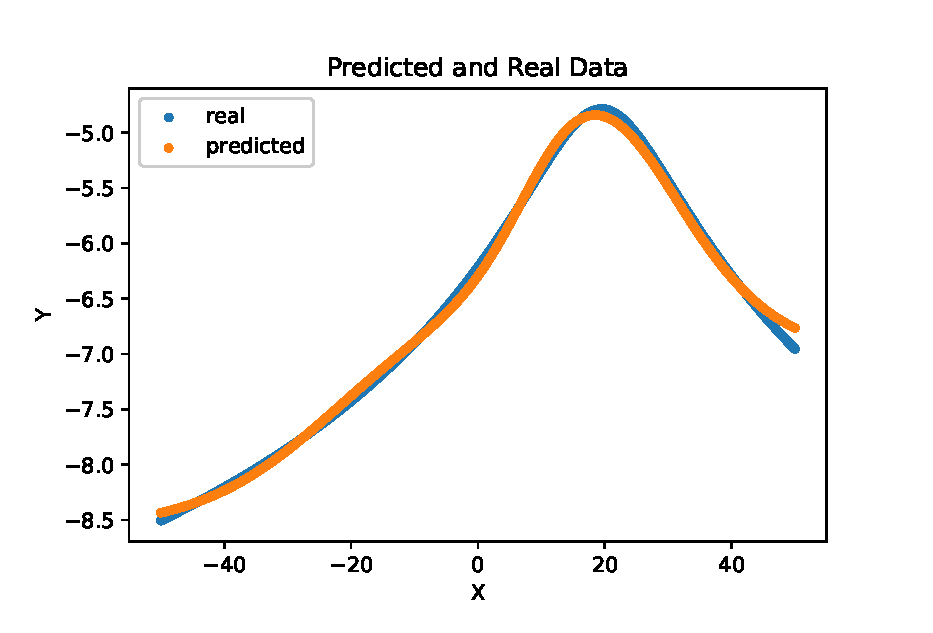
\includegraphics[scale=0.7]{multilayer_overfitted_new.eps}
  \caption{MLP Overfitting}
\end{figure}
\pagebreak

I personally was under lots of stress when I have been implementing this project. However, this model and the fitting that showed me made me happy. For all the weights, it is stored in file \texttt{overfit_weights.txt}. Also, The model had validation loss of 1.3 which is far less than that of section 4.6. This proves the fact that my program actually can fit MLP model into the data quite well. Since the real data and the predicted data from the model generated by my program was quite similar, we can safely say that we overfitted the model into the data as much as possible. Since I have proved that my model works, let's try to play with it with some various experiments. 

\subsubsection{Too Many Layers}
In our class time, we discussed something called "vanishing gradient". Which happens when a MLP gets too deep and each activation function's derivative getting multiplied lots of time eventually make the whole gradient go near 0. Therefore, I have also decided to see what happens if we stack too many layers into the model. I will be stacking 6 layers with sigmoid function as its activation function, as well as 2 identity functions. Also I trained them 50 epochs with learning rate of 0.01. Each layers had just one perceptron since I wanted a fast result that demonstrates the vanishing gradient effect. 

Before we actually test this thing out, we can kind of estimate what will happen if we stack too many layers. It is well known fact that sigmoid function's derivative has maximum value of 0.25. Meaning that if we stack one layer, the maximum value that the derivative can get is 0.25. If we stack 2 layers, the maximum value that those two layer's activation function's derivative multiplied is $0.25^2$. Therefore, after some layer $n$, the maximum value that the derivative can become is $0.25^n$. Therefore. the gradient will get close to 0. Now, let's see how it went. 

\begin{figure}[h]
  \centering
  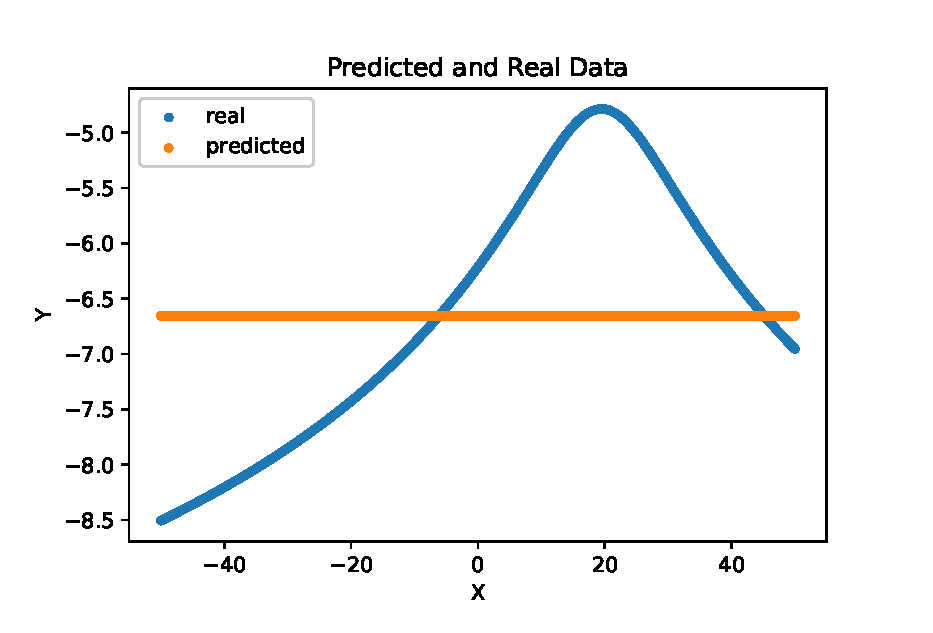
\includegraphics[scale=0.7]{multilayer_failure_1.eps}
  \caption{MLP Too Many Layers}
\end{figure}
\pagebreak

The regression model became a single line. Since each update values will become near 0, the model will have no meaning of weights. As we have expected, stacking too many layers will have bad effect on our overall model's performance. New lesson learned: stacking too many layers will not solve the problem. Also this will have a bad effect on the overall model's performance. Not only it had bad figure, it also had the worst validation loss which was roughly 723.

\subsubsection{Normal}

\begin{figure}[h]
  \centering
  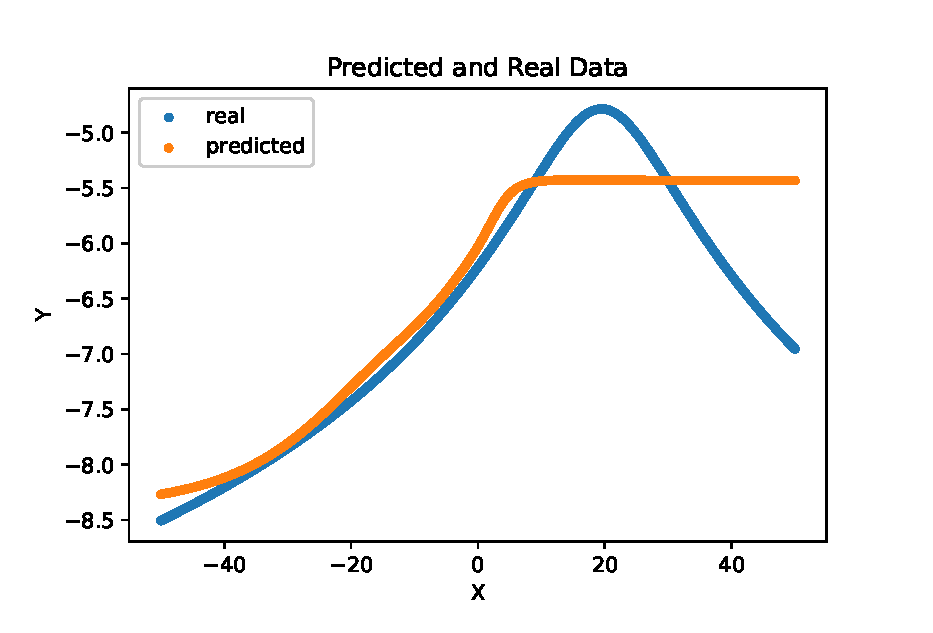
\includegraphics[scale=0.7]{multilayer_failure_normal.eps}
  \caption{MLP Normal Fit}
\end{figure}

Since we have seen some perfect fitting and a totally bad fitting, it's time for us to see some normal fittings. With most cases, this was the average normal case that I have encountered. In the beginning, it had a decent fit. However, after near $x=0$, it started to fit bad. As we all can see, from $x=0$ to $x=20$ roughly, the real data is above the model's prediction. Meanwhile, from $x=20$ to $x=40$, the real data is below the model's prediction. I consider this as the model falling into a local minimum. 

If we take a look at the loss function, we can kind of get a glimpse of what is happening. We have used the loss function as MSE. The deriviative of MSE will return following equation:
\[
    L^\prime(\hat{y}) = (\hat{y} - y)
\]

The model had validation loss of roughly 113, therefore performed worse than the overfitted case. MSE itself does not consider positive errors and negative errors. It just sums up all the error. However, with the derivative of MSE, negative and positive errors take into account. As we can see, from $x=0$ to $x=20$, the model will get a positive errors. Meanwhile, from $x=20$ to $x=40$, the model will get negative errors. Since the model has to minimize the total sum of positive errors and negative errors, the model decides to draw a line that makes the sum as small as possible. The model will fall into the pit of local optimum and will not think of fitting more into the data, instead it draws a line as the model. Therefore, I consider this as a typical local minimum problem.

The one of the most fundamental problem when it comes to using gradient descent as optimizer is falling into the local minimum. Therefore, we need to take other optimizers to escape from the local minimum and head to the global minimum. 

\subsubsection{Fine Tuning}
\label{sec:finetuning}
One of the problems that we have encountered in section 4.7.3 was the fact that we were using a static learning rate. It is well known fact that in the early stage of learning, we need bigger steps by bigger learning rate. However, as iterations go on, we need to decrease the step size by taking smaller learning rate. However, the our current model does not support this. Therefore, let's try to decrease learning rate after some iterations by ourselves. 

\begin{figure}[h]
    \centering
    \subfigure{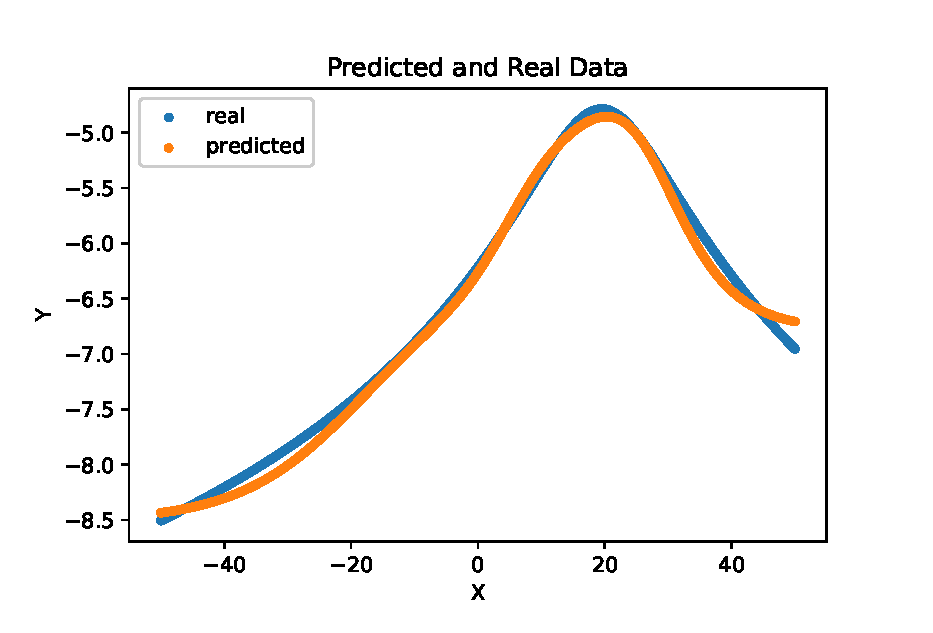
\includegraphics[scale=0.45]{multilayer_overfit_case2.eps}} 
    \subfigure{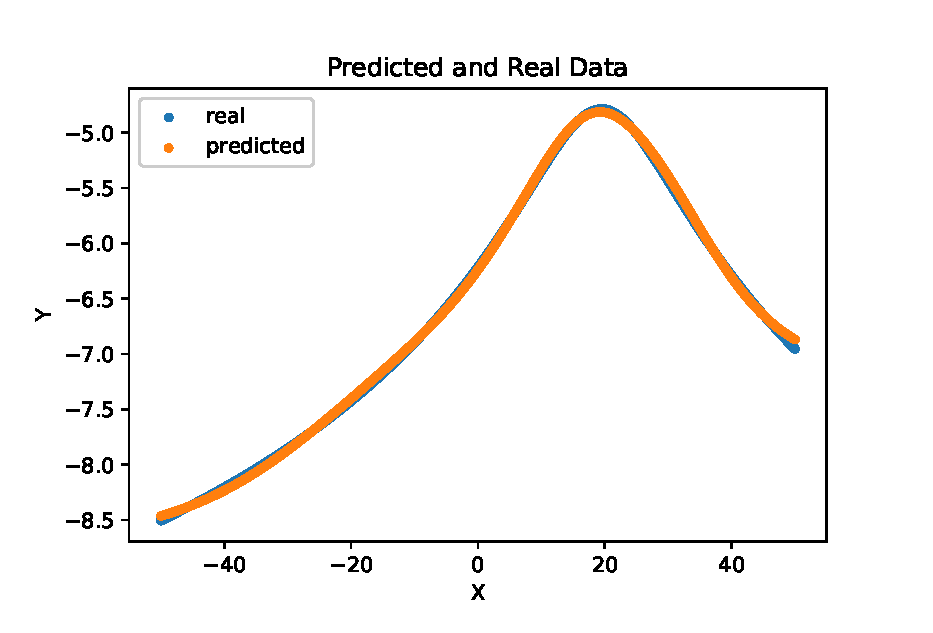
\includegraphics[scale=0.45]{multilayer_overfit_case6.eps}} 
    \caption{Fine Tuning}
\end{figure}

Left figure shows us the model after 50 epochs of learning rate using 0.01. With the left model, we were able to achieve a decent fitting. With the left model, I have trained the model with more iterations with smaller learning rate 0.001. As we all can see, the right figure was fit into the model far better than the original one. Let's see the training loss values with each model. Since as I wanted to overfit the model as much as possible, I did not split train and validation for this model. 

\begin{center}
\begin{table}[h]
\begin{tabularx}{1.0\textwidth} { 
  | >{\centering\arraybackslash}X 
  | >{\centering\arraybackslash}X | }
 \hline
 Before & After\\
 \hline
 21 & 1.16\\
    \hline
\end{tabularx}
\caption{Training Loss Comparison}
\end{table}
\end{center}
\pagebreak

The right model had almost no loss compared to the left model. With this experiment we can see that when a learning rate is fixed, it will have a bad effect on our model. The reason why this happens is due to the model swinging near the global minimum. With relatively big learning rate, the model will not get into the global minimum. In this experiment, I have manually tuned the learning rates. However, with real world workloads, we cannot do this. Therefore, we need to use some optimizers which support weight decaying.

\section{$N$ Hidden Layers with $M$ Perceptrons with \textit{ADAM}}
One of the most famous optimizer that supports weight decaying, as well as having a momentum which helps us escape local minimum, is \textit{ADAM}. Therefore, let's implement ADAM optimizer in our project. Since only the method \texttt{_back_propagate} in \texttt{Network} needs to be changed, this is quite easy to implement. Since the algorithm that \textit{ADAM} uses is well known, I will not mention how \textit{ADAM} works. The implementation of \textit{ADAM} can be found under the file \texttt{MultiLayer_Adam.ipynb}. 

In order to implement \textit{ADAM}, \texttt{Weight} and \texttt{Network._back_propagate} was redefined. For class \texttt{Weight}, some new attributes were defined:

\begin{itemize}
    \item \texttt{last_m}: The value that stores $m$. This is for storing the momentum before current training.
    \item \texttt{last_v}: The value that stores $v$. This is for storing the sum of gradient squared.
    \item \texttt{t}: The $t$ value. This is required for weight decay and $\hat{m}$ and $\hat{v}$ calibration. 
\end{itemize}


\texttt{Network._back_propagate} was redefined accordingly as well. In the original \textit{ADAM}'s paper, the authors suggested the following: "... Good default settings for the tested machine learning problems are $\alpha = 0.001$, $\beta1 = 0.9$, $\beta2 = 0.999$ and $\epsilon = 10^{-8}$ ..."

Therefore I used the same arguments as well. The method \texttt{Network.fit} was redefined like following example:
\\
\begin{center}
\begin{code}
\begin{minted}[frame=single,framesep=10pt]{python}
>> n1.fit(x, y, 50, 0.001, 0.9, 0.999, 10 ** -8)
Epoch 0 / 50 / Loss : 8.287144425690004e+02
Epoch 1 / 50 / Loss : 7.727202311870944e+02
Epoch 2 / 50 / Loss : 7.603810148305481e+02
Epoch 3 / 50 / Loss : 7.480318960704072e+02
...
\end{minted}
\captionof{listing}{\textit{ADAM} Implementation with MLP}
\end{code}
\end{center}

With 2 layers of sigmoid and a layer of linear function as activation functions, with 5 perceptrons each, I was able to get following result.

\pagebreak

\begin{figure}[h]
  \centering
  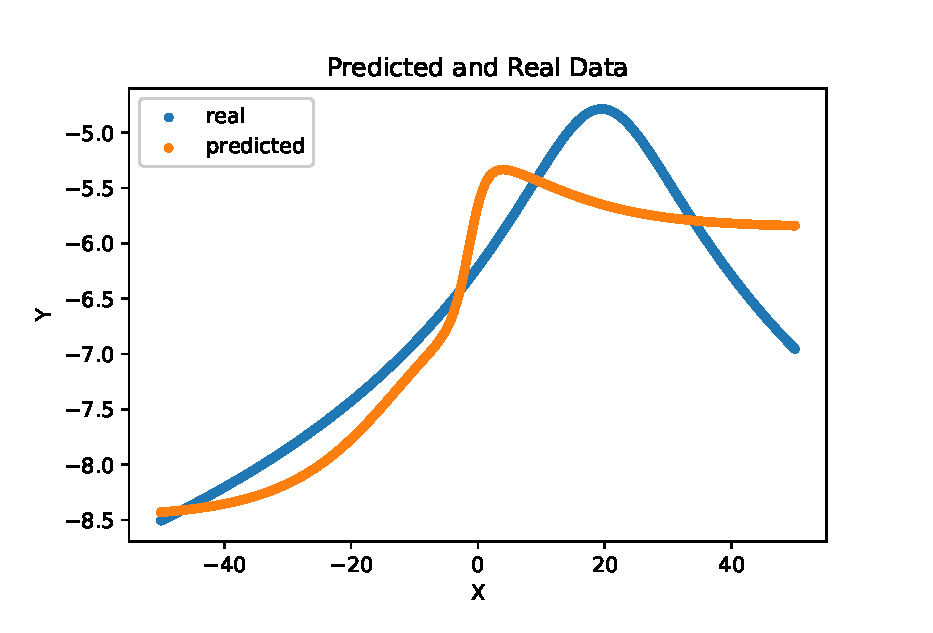
\includegraphics[scale=0.7]{multilayer_adam_new_1.eps}
  \caption{MLP ADAM Optimizer}
\end{figure}

The figure is quite satisfying. Although it had some weird fitting near $x=0$, it was quite reasonable fit. Of course, Since ADAM requires more calculation when it comes to updating weights, it took more time compared to the original gradient descent. However, there seemed to be a problem with this model.
\\

\begin{center}
\begin{code}
\begin{minted}[frame=single,framesep=10pt]{python}
...
Epoch 29 / 50  Loss : 4.063746920931958e+02
Epoch 30 / 50  Loss : 4.0799809029059594e+02
Epoch 31 / 50  Loss : 4.1283543336512446e+02
Epoch 32 / 50  Loss : 4.1956737870057435e+02
Epoch 33 / 50  Loss : 4.267237096477576e+02
...
\end{minted}
\captionof{listing}{\textit{ADAM} Problem}
\end{code}
\end{center}

With some epochs, the model got into a state that training loss was increasing. The problem seemed to be $\alpha$ being too big at the moment. Therefore, after first 50 epochs, I have set $\alpha=0.0001$ for better result. Then after another 300 epochs, following figure was the final output. I have also attached \texttt{adam_fit.gif} that shows the animation of fitting model using this program in each epochs. (Unfortunately Overleaf does not support \texttt{.gif} embedding to the document, so I had to attach it separately).

\pagebreak
\begin{figure}[h]
  \centering
  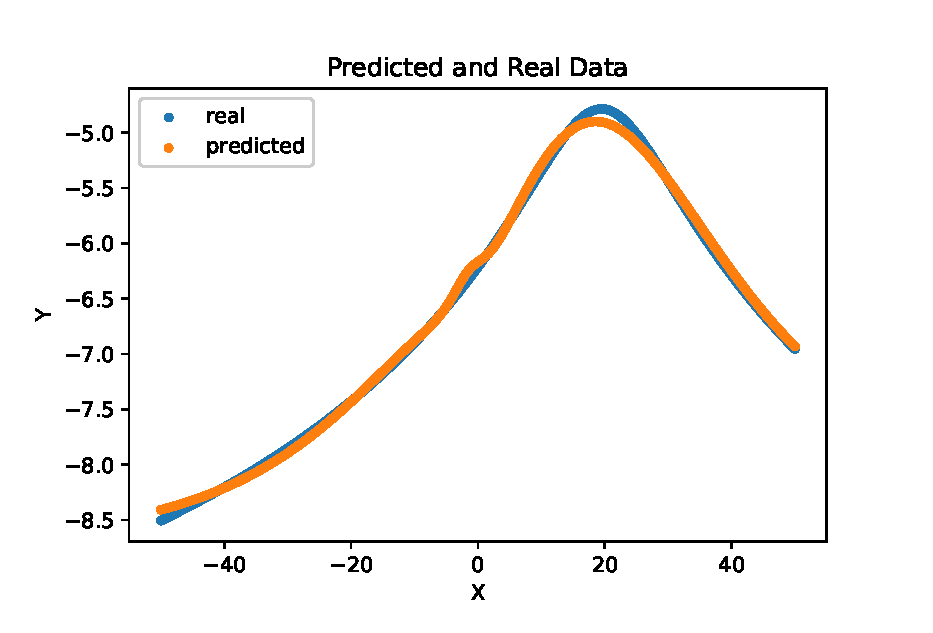
\includegraphics[scale=0.7]{multilayer_adam_new_5.eps}
  \caption{MLP ADAM Optimizer}
\end{figure}

So if we compare all models by validation loss, we can retrieve a simple table like below:

\begin{center}
\begin{table}[h]
\begin{tabularx}{1.0\textwidth} { 
  | >{\centering\arraybackslash}X 
| >{\centering\arraybackslash}X 
  | >{\centering\arraybackslash}X 
  | >{\centering\arraybackslash}X 
    | >{\centering\arraybackslash}X 
  | >{\centering\arraybackslash}X | }
 \hline
 First Implementation & Single Layer & Overfitted & Normal Fit & Too Many Layers & ADAM \\
 \hline
 104 & 63 & 1.3 & 723 & 113 & ?\\
    \hline
\end{tabularx}
\caption{Training Loss Comparison}
\end{table}
\end{center}

It is quite interesting to me that even with same network model, with different arguments the result varies so much. If we select good arguments like decent number of perceptrons and appropriate activation functions, we can almost overfit the whole model into the data. However, if we select bad activation functions and stack too many layers, the performance gets damaged a lot.

Also selecting a good optimizer algorithm was important as well. Since just using gradient descent would make the model get stuck in the local minimum, selecting a good optimizer like ADAM will help the model escape local minimum. 

\pagebreak
\section{Conclusion}
Implementing MLP was fun. While implementing this project, I was able to learn following things:

\subsection{Layers}
Stacking layers is always not the solution. At first, stacking multiple layers seemed to solve the problem. However, when testing multiple conditions, this turned out not to be the case. With more layers, there is a bit of performance boost. Stacking an appropriate amount of layers help our model fit into the given data. However, stacking too much will be a cause for vanishing gradient problem as well as long training time or even train a wrong model.

\subsection{Perceptrons}
Using more perceptrons per layers is not always the solution as well. This looked a promising solution when I first encountered this project. However, with many layers, the training time increases. For example, if we have $n$ perceptron per layers, and if we stack $m$ layers, this will give us $n^m$ weights to train. Not only this is a big number of weights to train, but it also takes much time when backpropagating.

\subsection{Learning Rate}
Choosing good learning rate is important. If a learning rate is too small, it will make the whole model train slower. However, with too big learning rate, it has high chance of "swinging" gradients. Also, using a static value of learning rate is not ideal. Therefore, weight decaying is required to reduce learning rate automatically after epochs. 

\subsection{Optimizer}
Gradient descent is not perfect, as we all know. Although gradient descent is easy to implement and intuitive, it has high potential of falling into local minimum. Due to the characteristics of gradient descent, this is inevitable. Therefore, using other optimizers such as \textit{AdaGrad}, \textit{Adam}, etc will be a better choice. Also, as we have seen in the section \hyperref[finetuning]{section 4.4}, we need to make a dynamic learning rate. Keeping a static learning rate is bad for the model's overall performance.

\subsection{Conclusion}
Although the project was difficult and hard to implement at first, however watching my model fit perfectly into the data was so satisfying. When I was taking the class, there were some tips that professor told us. However, frankly speaking, I did listen to those tips however did not feel the need to really follow those tips. While testing with various settings in this project, I encountered those tips were very useful. Such include need of good optimizer and choosing a good learning rate. Learned lots of good things by this project. 
\end{document}


